\documentclass[1p]{elsarticle_modified}
%\bibliographystyle{elsarticle-num}

%\usepackage[colorlinks]{hyperref}
%\usepackage{abbrmath_seonhwa} %\Abb, \Ascr, \Acal ,\Abf, \Afrak
\usepackage{amsfonts}
\usepackage{amssymb}
\usepackage{amsmath}
\usepackage{amsthm}
\usepackage{scalefnt}
\usepackage{amsbsy}
\usepackage{kotex}
\usepackage{caption}
\usepackage{subfig}
\usepackage{color}
\usepackage{graphicx}
\usepackage{xcolor} %% white, black, red, green, blue, cyan, magenta, yellow
\usepackage{float}
\usepackage{setspace}
\usepackage{hyperref}

\usepackage{tikz}
\usetikzlibrary{arrows}

\usepackage{multirow}
\usepackage{array} % fixed length table
\usepackage{hhline}

%%%%%%%%%%%%%%%%%%%%%
\makeatletter
\renewcommand*\env@matrix[1][\arraystretch]{%
	\edef\arraystretch{#1}%
	\hskip -\arraycolsep
	\let\@ifnextchar\new@ifnextchar
	\array{*\c@MaxMatrixCols c}}
\makeatother %https://tex.stackexchange.com/questions/14071/how-can-i-increase-the-line-spacing-in-a-matrix
%%%%%%%%%%%%%%%

\usepackage[normalem]{ulem}

\newcommand{\msout}[1]{\ifmmode\text{\sout{\ensuremath{#1}}}\else\sout{#1}\fi}
%SOURCE: \msout is \stkout macro in https://tex.stackexchange.com/questions/20609/strikeout-in-math-mode

\newcommand{\cancel}[1]{
	\ifmmode
	{\color{red}\msout{#1}}
	\else
	{\color{red}\sout{#1}}
	\fi
}

\newcommand{\add}[1]{
	{\color{blue}\uwave{#1}}
}

\newcommand{\replace}[2]{
	\ifmmode
	{\color{red}\msout{#1}}{\color{blue}\uwave{#2}}
	\else
	{\color{red}\sout{#1}}{\color{blue}\uwave{#2}}
	\fi
}

\newcommand{\Sol}{\mathcal{S}} %segment
\newcommand{\D}{D} %diagram
\newcommand{\A}{\mathcal{A}} %arc


%%%%%%%%%%%%%%%%%%%%%%%%%%%%%5 test

\def\sl{\operatorname{\textup{SL}}(2,\Cbb)}
\def\psl{\operatorname{\textup{PSL}}(2,\Cbb)}
\def\quan{\mkern 1mu \triangleright \mkern 1mu}

\theoremstyle{definition}
\newtheorem{thm}{Theorem}[section]
\newtheorem{prop}[thm]{Proposition}
\newtheorem{lem}[thm]{Lemma}
\newtheorem{ques}[thm]{Question}
\newtheorem{cor}[thm]{Corollary}
\newtheorem{defn}[thm]{Definition}
\newtheorem{exam}[thm]{Example}
\newtheorem{rmk}[thm]{Remark}
\newtheorem{alg}[thm]{Algorithm}

\newcommand{\I}{\sqrt{-1}}
\begin{document}

%\begin{frontmatter}
%
%\title{Boundary parabolic representations of knots up to 8 crossings}
%
%%% Group authors per affiliation:
%\author{Yunhi Cho} 
%\address{Department of Mathematics, University of Seoul, Seoul, Korea}
%\ead{yhcho@uos.ac.kr}
%
%
%\author{Seonhwa Kim} %\fnref{s_kim}}
%\address{Center for Geometry and Physics, Institute for Basic Science, Pohang, 37673, Korea}
%\ead{ryeona17@ibs.re.kr}
%
%\author{Hyuk Kim}
%\address{Department of Mathematical Sciences, Seoul National University, Seoul 08826, Korea}
%\ead{hyukkim@snu.ac.kr}
%
%\author{Seokbeom Yoon}
%\address{Department of Mathematical Sciences, Seoul National University, Seoul, 08826,  Korea}
%\ead{sbyoon15@snu.ac.kr}
%
%\begin{abstract}
%We find all boundary parabolic representation of knots up to 8 crossings.
%
%\end{abstract}
%\begin{keyword}
%    \MSC[2010] 57M25 
%\end{keyword}
%
%\end{frontmatter}

%\linenumbers
%\tableofcontents
%
\newcommand\colored[1]{\textcolor{white}{\rule[-0.35ex]{0.8em}{1.4ex}}\kern-0.8em\color{red} #1}%
%\newcommand\colored[1]{\textcolor{white}{ #1}\kern-2.17ex	\textcolor{white}{ #1}\kern-1.81ex	\textcolor{white}{ #1}\kern-2.15ex\color{red}#1	}

{\Large $\underline{12n_{0303}~(K12n_{0303})}$}

\setlength{\tabcolsep}{10pt}
\renewcommand{\arraystretch}{1.6}
\vspace{1cm}\begin{tabular}{m{100pt}>{\centering\arraybackslash}m{274pt}}
\multirow{5}{120pt}{
	\centering
	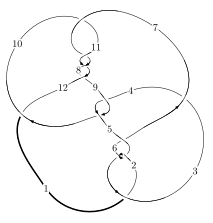
\includegraphics[width=112pt]{../../../GIT/diagram.site/Diagrams/png/2392_12n_0303.png}\\
\ \ \ A knot diagram\footnotemark}&
\allowdisplaybreaks
\textbf{Linearized knot diagam} \\
\cline{2-2}
 &
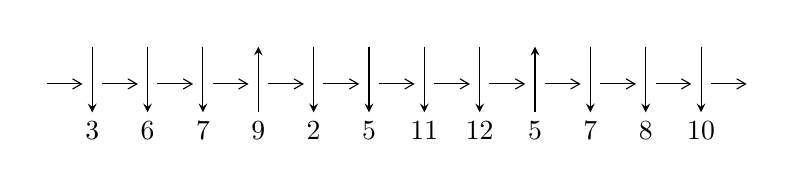
\begin{tikzpicture}[x=20pt, y=17pt]
	% nodes
	\node (C0) at (0, 0) {};
	\node (C1) at (1, 0) {};
	\node (C1U) at (1, +1) {};
	\node (C1D) at (1, -1) {3};

	\node (C2) at (2, 0) {};
	\node (C2U) at (2, +1) {};
	\node (C2D) at (2, -1) {6};

	\node (C3) at (3, 0) {};
	\node (C3U) at (3, +1) {};
	\node (C3D) at (3, -1) {7};

	\node (C4) at (4, 0) {};
	\node (C4U) at (4, +1) {};
	\node (C4D) at (4, -1) {9};

	\node (C5) at (5, 0) {};
	\node (C5U) at (5, +1) {};
	\node (C5D) at (5, -1) {2};

	\node (C6) at (6, 0) {};
	\node (C6U) at (6, +1) {};
	\node (C6D) at (6, -1) {5};

	\node (C7) at (7, 0) {};
	\node (C7U) at (7, +1) {};
	\node (C7D) at (7, -1) {11};

	\node (C8) at (8, 0) {};
	\node (C8U) at (8, +1) {};
	\node (C8D) at (8, -1) {12};

	\node (C9) at (9, 0) {};
	\node (C9U) at (9, +1) {};
	\node (C9D) at (9, -1) {5};

	\node (C10) at (10, 0) {};
	\node (C10U) at (10, +1) {};
	\node (C10D) at (10, -1) {7};

	\node (C11) at (11, 0) {};
	\node (C11U) at (11, +1) {};
	\node (C11D) at (11, -1) {8};

	\node (C12) at (12, 0) {};
	\node (C12U) at (12, +1) {};
	\node (C12D) at (12, -1) {10};
	\node (C13) at (13, 0) {};

	% arrows
	\draw[->,>={angle 60}]
	(C0) edge (C1) (C1) edge (C2) (C2) edge (C3) (C3) edge (C4) (C4) edge (C5) (C5) edge (C6) (C6) edge (C7) (C7) edge (C8) (C8) edge (C9) (C9) edge (C10) (C10) edge (C11) (C11) edge (C12) (C12) edge (C13) ;	\draw[->,>=stealth]
	(C1U) edge (C1D) (C2U) edge (C2D) (C3U) edge (C3D) (C4D) edge (C4U) (C5U) edge (C5D) (C6U) edge (C6D) (C7U) edge (C7D) (C8U) edge (C8D) (C9D) edge (C9U) (C10U) edge (C10D) (C11U) edge (C11D) (C12U) edge (C12D) ;
	\end{tikzpicture} \\
\hhline{~~} \\& 
\textbf{Solving Sequence} \\ \cline{2-2} 
 &
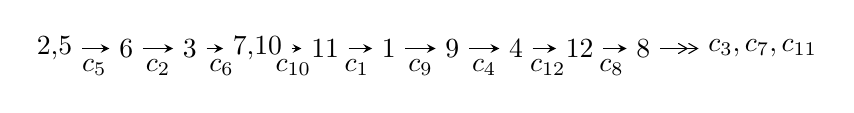
\begin{tikzpicture}[x=23pt, y=7pt]
	% node
	\node (A0) at (-1/8, 0) {2,5};
	\node (A1) at (1, 0) {6};
	\node (A2) at (2, 0) {3};
	\node (A3) at (49/16, 0) {7,10};
	\node (A4) at (33/8, 0) {11};
	\node (A5) at (41/8, 0) {1};
	\node (A6) at (49/8, 0) {9};
	\node (A7) at (57/8, 0) {4};
	\node (A8) at (65/8, 0) {12};
	\node (A9) at (73/8, 0) {8};
	\node (C1) at (1/2, -1) {$c_{5}$};
	\node (C2) at (3/2, -1) {$c_{2}$};
	\node (C3) at (5/2, -1) {$c_{6}$};
	\node (C4) at (29/8, -1) {$c_{10}$};
	\node (C5) at (37/8, -1) {$c_{1}$};
	\node (C6) at (45/8, -1) {$c_{9}$};
	\node (C7) at (53/8, -1) {$c_{4}$};
	\node (C8) at (61/8, -1) {$c_{12}$};
	\node (C9) at (69/8, -1) {$c_{8}$};
	\node (A10) at (11, 0) {$c_{3},c_{7},c_{11}$};

	% edge
	\draw[->,>=stealth]	
	(A0) edge (A1) (A1) edge (A2) (A2) edge (A3) (A3) edge (A4) (A4) edge (A5) (A5) edge (A6) (A6) edge (A7) (A7) edge (A8) (A8) edge (A9) ;
	\draw[->>,>={angle 60}]	
	(A9) edge (A10);
\end{tikzpicture} \\ 

\end{tabular} \\

\footnotetext{
The image of knot diagram is generated by the software ``\textbf{Draw programme}" developed by Andrew Bartholomew(\url{http://www.layer8.co.uk/maths/draw/index.htm\#Running-draw}), where we modified some parts for our purpose(\url{https://github.com/CATsTAILs/LinksPainter}).
}\phantom \\ \newline 
\centering \textbf{Ideals for irreducible components\footnotemark of $X_{\text{par}}$} 
 
\begin{align*}
I^u_{1}&=\langle 
u^{23}+u^{22}+\cdots+b-2 u,\;-3 u^{23}-6 u^{22}+\cdots+2 a+7,\;u^{26}+3 u^{25}+\cdots-9 u^2+1\rangle \\
I^u_{2}&=\langle 
b,\;a^2+a u- u^2- a+2 u-1,\;u^3- u^2+1\rangle \\
\\
\end{align*}
\raggedright * 2 irreducible components of $\dim_{\mathbb{C}}=0$, with total 32 representations.\\
\footnotetext{All coefficients of polynomials are rational numbers. But the coefficients are sometimes approximated in decimal forms when there is not enough margin.}
\newpage
\renewcommand{\arraystretch}{1}
\centering \section*{I. $I^u_{1}= \langle u^{23}+u^{22}+\cdots+b-2 u,\;-3 u^{23}-6 u^{22}+\cdots+2 a+7,\;u^{26}+3 u^{25}+\cdots-9 u^2+1 \rangle$}
\flushleft \textbf{(i) Arc colorings}\\
\begin{tabular}{m{7pt} m{180pt} m{7pt} m{180pt} }
\flushright $a_{2}=$&$\begin{pmatrix}0\\u\end{pmatrix}$ \\
\flushright $a_{5}=$&$\begin{pmatrix}1\\0\end{pmatrix}$ \\
\flushright $a_{6}=$&$\begin{pmatrix}1\\u^2\end{pmatrix}$ \\
\flushright $a_{3}=$&$\begin{pmatrix}- u\\- u^3+u\end{pmatrix}$ \\
\flushright $a_{7}=$&$\begin{pmatrix}- u^2+1\\u^2\end{pmatrix}$ \\
\flushright $a_{10}=$&$\begin{pmatrix}\frac{3}{2} u^{23}+3 u^{22}+\cdots-4 u-\frac{7}{2}\\- u^{23}- u^{22}+\cdots+2 u^2+2 u\end{pmatrix}$ \\
\flushright $a_{11}=$&$\begin{pmatrix}u^{25}+\frac{7}{2} u^{24}+\cdots-\frac{11}{2} u-3\\-\frac{1}{2} u^{25}-\frac{3}{2} u^{24}+\cdots+\frac{3}{2} u-\frac{1}{2}\end{pmatrix}$ \\
\flushright $a_{1}=$&$\begin{pmatrix}u^3\\u^5- u^3+u\end{pmatrix}$ \\
\flushright $a_{9}=$&$\begin{pmatrix}\frac{5}{2} u^{23}+4 u^{22}+\cdots-6 u-\frac{7}{2}\\- u^{23}- u^{22}+\cdots+2 u^2+2 u\end{pmatrix}$ \\
\flushright $a_{4}=$&$\begin{pmatrix}u^7-2 u^5+2 u^3-2 u\\- u^7+u^5-2 u^3+u\end{pmatrix}$ \\
\flushright $a_{12}=$&$\begin{pmatrix}\frac{1}{2} u^{23}+u^{22}+\cdots+2 u+\frac{1}{2}\\- u^2\end{pmatrix}$ \\
\flushright $a_{8}=$&$\begin{pmatrix}\frac{1}{2} u^{24}-2 u^{22}+\cdots-\frac{7}{2} u+1\\-\frac{1}{2} u^{25}-\frac{3}{2} u^{24}+\cdots+\frac{3}{2} u-\frac{1}{2}\end{pmatrix}$\\&\end{tabular}
\flushleft \textbf{(ii) Obstruction class $= -1$}\\~\\
\flushleft \textbf{(iii) Cusp Shapes $= -\frac{11}{2} u^{25}-12 u^{24}+\frac{1}{2} u^{23}+30 u^{22}-13 u^{21}-105 u^{20}-42 u^{19}+\frac{337}{2} u^{18}+57 u^{17}-325 u^{16}-196 u^{15}+356 u^{14}+198 u^{13}-\frac{979}{2} u^{12}-283 u^{11}+\frac{789}{2} u^{10}+\frac{353}{2} u^9-\frac{809}{2} u^8-\frac{297}{2} u^7+250 u^6+41 u^5-154 u^4-16 u^3+\frac{149}{2} u^2+13 u-\frac{33}{2}$}\\~\\
\newpage\renewcommand{\arraystretch}{1}
\flushleft \textbf{(iv) u-Polynomials at the component}\newline \\
\begin{tabular}{m{50pt}|m{274pt}}
Crossings & \hspace{64pt}u-Polynomials at each crossing \\
\hline $$\begin{aligned}c_{1},c_{6}\end{aligned}$$&$\begin{aligned}
&u^{26}+5 u^{25}+\cdots+18 u+1
\end{aligned}$\\
\hline $$\begin{aligned}c_{2},c_{5}\end{aligned}$$&$\begin{aligned}
&u^{26}+3 u^{25}+\cdots-9 u^2+1
\end{aligned}$\\
\hline $$\begin{aligned}c_{3}\end{aligned}$$&$\begin{aligned}
&u^{26}-3 u^{25}+\cdots+6516 u+1009
\end{aligned}$\\
\hline $$\begin{aligned}c_{4},c_{9}\end{aligned}$$&$\begin{aligned}
&u^{26}- u^{25}+\cdots+96 u+64
\end{aligned}$\\
\hline $$\begin{aligned}c_{7},c_{8},c_{10}\\c_{11}\end{aligned}$$&$\begin{aligned}
&u^{26}+4 u^{25}+\cdots-3 u+1
\end{aligned}$\\
\hline $$\begin{aligned}c_{12}\end{aligned}$$&$\begin{aligned}
&u^{26}+28 u^{24}+\cdots-31 u-1
\end{aligned}$\\
\hline
\end{tabular}\\~\\
\newpage\renewcommand{\arraystretch}{1}
\flushleft \textbf{(v) Riley Polynomials at the component}\newline \\
\begin{tabular}{m{50pt}|m{274pt}}
Crossings & \hspace{64pt}Riley Polynomials at each crossing \\
\hline $$\begin{aligned}c_{1},c_{6}\end{aligned}$$&$\begin{aligned}
&y^{26}+35 y^{25}+\cdots-74 y+1
\end{aligned}$\\
\hline $$\begin{aligned}c_{2},c_{5}\end{aligned}$$&$\begin{aligned}
&y^{26}-5 y^{25}+\cdots-18 y+1
\end{aligned}$\\
\hline $$\begin{aligned}c_{3}\end{aligned}$$&$\begin{aligned}
&y^{26}+95 y^{25}+\cdots-36103574 y+1018081
\end{aligned}$\\
\hline $$\begin{aligned}c_{4},c_{9}\end{aligned}$$&$\begin{aligned}
&y^{26}-35 y^{25}+\cdots-58368 y+4096
\end{aligned}$\\
\hline $$\begin{aligned}c_{7},c_{8},c_{10}\\c_{11}\end{aligned}$$&$\begin{aligned}
&y^{26}-28 y^{25}+\cdots-27 y+1
\end{aligned}$\\
\hline $$\begin{aligned}c_{12}\end{aligned}$$&$\begin{aligned}
&y^{26}+56 y^{25}+\cdots-391 y+1
\end{aligned}$\\
\hline
\end{tabular}\\~\\
\newpage\flushleft \textbf{(vi) Complex Volumes and Cusp Shapes}
$$\begin{array}{c|c|c}  
\text{Solutions to }I^u_{1}& \I (\text{vol} + \sqrt{-1}CS) & \text{Cusp shape}\\
 \hline 
\begin{aligned}
u &= \phantom{-}0.697878 + 0.750786 I \\
a &= \phantom{-}0.950274 + 0.282069 I \\
b &= -0.969430 + 0.478608 I\end{aligned}
 & \phantom{-}3.30312 - 1.30372 I & -2.90180 + 1.28901 I \\ \hline\begin{aligned}
u &= \phantom{-}0.697878 - 0.750786 I \\
a &= \phantom{-}0.950274 - 0.282069 I \\
b &= -0.969430 - 0.478608 I\end{aligned}
 & \phantom{-}3.30312 + 1.30372 I & -2.90180 - 1.28901 I \\ \hline\begin{aligned}
u &= -1.05556\phantom{ +0.000000I} \\
a &= -1.13582\phantom{ +0.000000I} \\
b &= -1.20261\phantom{ +0.000000I}\end{aligned}
 & -6.55918\phantom{ +0.000000I} & -13.9020\phantom{ +0.000000I} \\ \hline\begin{aligned}
u &= -0.714104 + 0.530028 I \\
a &= -0.308272 + 1.024340 I \\
b &= -0.222426 + 0.888370 I\end{aligned}
 & -7.39553 + 1.99902 I & -12.68261 - 2.64464 I \\ \hline\begin{aligned}
u &= -0.714104 - 0.530028 I \\
a &= -0.308272 - 1.024340 I \\
b &= -0.222426 - 0.888370 I\end{aligned}
 & -7.39553 - 1.99902 I & -12.68261 + 2.64464 I \\ \hline\begin{aligned}
u &= \phantom{-}0.426539 + 0.776149 I \\
a &= -1.244140 - 0.230526 I \\
b &= \phantom{-}1.405990 + 0.009237 I\end{aligned}
 & -1.37386 + 1.46827 I & -7.40504 - 0.61110 I \\ \hline\begin{aligned}
u &= \phantom{-}0.426539 - 0.776149 I \\
a &= -1.244140 + 0.230526 I \\
b &= \phantom{-}1.405990 - 0.009237 I\end{aligned}
 & -1.37386 - 1.46827 I & -7.40504 + 0.61110 I \\ \hline\begin{aligned}
u &= \phantom{-}0.924653 + 0.644299 I \\
a &= -0.192140 - 0.877647 I \\
b &= \phantom{-}0.922849 + 0.070450 I\end{aligned}
 & \phantom{-}2.53585 - 3.91698 I & -4.21369 + 6.80514 I \\ \hline\begin{aligned}
u &= \phantom{-}0.924653 - 0.644299 I \\
a &= -0.192140 + 0.877647 I \\
b &= \phantom{-}0.922849 - 0.070450 I\end{aligned}
 & \phantom{-}2.53585 + 3.91698 I & -4.21369 - 6.80514 I \\ \hline\begin{aligned}
u &= \phantom{-}1.032140 + 0.523292 I \\
a &= \phantom{-}0.16264 + 1.48931 I \\
b &= -1.372650 + 0.239227 I\end{aligned}
 & -3.36202 - 6.28703 I & -10.76890 + 5.79025 I\\
 \hline 
 \end{array}$$\newpage$$\begin{array}{c|c|c}  
\text{Solutions to }I^u_{1}& \I (\text{vol} + \sqrt{-1}CS) & \text{Cusp shape}\\
 \hline 
\begin{aligned}
u &= \phantom{-}1.032140 - 0.523292 I \\
a &= \phantom{-}0.16264 - 1.48931 I \\
b &= -1.372650 - 0.239227 I\end{aligned}
 & -3.36202 + 6.28703 I & -10.76890 - 5.79025 I \\ \hline\begin{aligned}
u &= -0.826543\phantom{ +0.000000I} \\
a &= \phantom{-}0.499620\phantom{ +0.000000I} \\
b &= \phantom{-}0.424946\phantom{ +0.000000I}\end{aligned}
 & -1.35750\phantom{ +0.000000I} & -5.74160\phantom{ +0.000000I} \\ \hline\begin{aligned}
u &= \phantom{-}0.904709 + 0.855635 I \\
a &= -0.749040 + 0.396223 I \\
b &= \phantom{-}0.015583 - 1.255880 I\end{aligned}
 & \phantom{-}0.45711 - 3.16518 I & -10.09379 + 2.71963 I \\ \hline\begin{aligned}
u &= \phantom{-}0.904709 - 0.855635 I \\
a &= -0.749040 - 0.396223 I \\
b &= \phantom{-}0.015583 + 1.255880 I\end{aligned}
 & \phantom{-}0.45711 + 3.16518 I & -10.09379 - 2.71963 I \\ \hline\begin{aligned}
u &= -0.874451 + 0.958708 I \\
a &= -1.34597 + 0.77169 I \\
b &= \phantom{-}1.85003 - 0.54896 I\end{aligned}
 & \phantom{-}6.92052 - 3.79217 I & -7.74212 + 0.87029 I \\ \hline\begin{aligned}
u &= -0.874451 - 0.958708 I \\
a &= -1.34597 - 0.77169 I \\
b &= \phantom{-}1.85003 + 0.54896 I\end{aligned}
 & \phantom{-}6.92052 + 3.79217 I & -7.74212 - 0.87029 I \\ \hline\begin{aligned}
u &= -0.932825 + 0.952507 I \\
a &= \phantom{-}1.48560 - 0.97786 I \\
b &= -2.02844 + 0.13031 I\end{aligned}
 & \phantom{-}13.70930 + 0.63054 I & -5.09956 + 0.08472 I \\ \hline\begin{aligned}
u &= -0.932825 - 0.952507 I \\
a &= \phantom{-}1.48560 + 0.97786 I \\
b &= -2.02844 - 0.13031 I\end{aligned}
 & \phantom{-}13.70930 - 0.63054 I & -5.09956 - 0.08472 I \\ \hline\begin{aligned}
u &= -1.007520 + 0.885407 I \\
a &= \phantom{-}1.72924 - 1.22466 I \\
b &= -1.78041 - 0.65102 I\end{aligned}
 & \phantom{-}6.48279 + 10.56660 I & -8.37835 - 5.32202 I \\ \hline\begin{aligned}
u &= -1.007520 - 0.885407 I \\
a &= \phantom{-}1.72924 + 1.22466 I \\
b &= -1.78041 + 0.65102 I\end{aligned}
 & \phantom{-}6.48279 - 10.56660 I & -8.37835 + 5.32202 I\\
 \hline 
 \end{array}$$\newpage$$\begin{array}{c|c|c}  
\text{Solutions to }I^u_{1}& \I (\text{vol} + \sqrt{-1}CS) & \text{Cusp shape}\\
 \hline 
\begin{aligned}
u &= -0.977518 + 0.926314 I \\
a &= -1.61355 + 1.11637 I \\
b &= \phantom{-}1.99598 + 0.29162 I\end{aligned}
 & \phantom{-}13.5604 + 6.2675 I & -5.43427 - 4.61670 I \\ \hline\begin{aligned}
u &= -0.977518 - 0.926314 I \\
a &= -1.61355 - 1.11637 I \\
b &= \phantom{-}1.99598 - 0.29162 I\end{aligned}
 & \phantom{-}13.5604 - 6.2675 I & -5.43427 + 4.61670 I \\ \hline\begin{aligned}
u &= \phantom{-}0.605940\phantom{ +0.000000I} \\
a &= \phantom{-}3.65946\phantom{ +0.000000I} \\
b &= -0.461168\phantom{ +0.000000I}\end{aligned}
 & -9.68489\phantom{ +0.000000I} & \phantom{-}0.985630\phantom{ +0.000000I} \\ \hline\begin{aligned}
u &= -0.507505 + 0.285828 I \\
a &= \phantom{-}0.417815 - 0.836271 I \\
b &= \phantom{-}0.046187 - 0.679181 I\end{aligned}
 & -0.698170 + 0.981366 I & -8.43360 - 6.86703 I \\ \hline\begin{aligned}
u &= -0.507505 - 0.285828 I \\
a &= \phantom{-}0.417815 + 0.836271 I \\
b &= \phantom{-}0.046187 + 0.679181 I\end{aligned}
 & -0.698170 - 0.981366 I & -8.43360 + 6.86703 I \\ \hline\begin{aligned}
u &= \phantom{-}0.332169\phantom{ +0.000000I} \\
a &= -2.60819\phantom{ +0.000000I} \\
b &= \phantom{-}0.512315\phantom{ +0.000000I}\end{aligned}
 & -1.32945\phantom{ +0.000000I} & -6.03470\phantom{ +0.000000I}\\
 \hline 
 \end{array}$$\newpage\newpage\renewcommand{\arraystretch}{1}
\centering \section*{II. $I^u_{2}= \langle b,\;a^2+a u- u^2- a+2 u-1,\;u^3- u^2+1 \rangle$}
\flushleft \textbf{(i) Arc colorings}\\
\begin{tabular}{m{7pt} m{180pt} m{7pt} m{180pt} }
\flushright $a_{2}=$&$\begin{pmatrix}0\\u\end{pmatrix}$ \\
\flushright $a_{5}=$&$\begin{pmatrix}1\\0\end{pmatrix}$ \\
\flushright $a_{6}=$&$\begin{pmatrix}1\\u^2\end{pmatrix}$ \\
\flushright $a_{3}=$&$\begin{pmatrix}- u\\- u^2+u+1\end{pmatrix}$ \\
\flushright $a_{7}=$&$\begin{pmatrix}- u^2+1\\u^2\end{pmatrix}$ \\
\flushright $a_{10}=$&$\begin{pmatrix}a\\0\end{pmatrix}$ \\
\flushright $a_{11}=$&$\begin{pmatrix}a u+2 a\\u^2 a- a u- a\end{pmatrix}$ \\
\flushright $a_{1}=$&$\begin{pmatrix}u^2-1\\- u^2\end{pmatrix}$ \\
\flushright $a_{9}=$&$\begin{pmatrix}a\\0\end{pmatrix}$ \\
\flushright $a_{4}=$&$\begin{pmatrix}1\\0\end{pmatrix}$ \\
\flushright $a_{12}=$&$\begin{pmatrix}u^2- a+u-2\\- u^2\end{pmatrix}$ \\
\flushright $a_{8}=$&$\begin{pmatrix}- a u-2 a+u-1\\- u^2 a+a u+a\end{pmatrix}$\\&\end{tabular}
\flushleft \textbf{(ii) Obstruction class $= 1$}\\~\\
\flushleft \textbf{(iii) Cusp Shapes $= - u^2 a-3 u^2- a+8 u-13$}\\~\\
\newpage\renewcommand{\arraystretch}{1}
\flushleft \textbf{(iv) u-Polynomials at the component}\newline \\
\begin{tabular}{m{50pt}|m{274pt}}
Crossings & \hspace{64pt}u-Polynomials at each crossing \\
\hline $$\begin{aligned}c_{1},c_{3}\end{aligned}$$&$\begin{aligned}
&(u^3- u^2+2 u-1)^2
\end{aligned}$\\
\hline $$\begin{aligned}c_{2}\end{aligned}$$&$\begin{aligned}
&(u^3+u^2-1)^2
\end{aligned}$\\
\hline $$\begin{aligned}c_{4},c_{9}\end{aligned}$$&$\begin{aligned}
&u^6
\end{aligned}$\\
\hline $$\begin{aligned}c_{5}\end{aligned}$$&$\begin{aligned}
&(u^3- u^2+1)^2
\end{aligned}$\\
\hline $$\begin{aligned}c_{6}\end{aligned}$$&$\begin{aligned}
&(u^3+u^2+2 u+1)^2
\end{aligned}$\\
\hline $$\begin{aligned}c_{7},c_{8}\end{aligned}$$&$\begin{aligned}
&(u^2+u-1)^3
\end{aligned}$\\
\hline $$\begin{aligned}c_{10},c_{11},c_{12}\end{aligned}$$&$\begin{aligned}
&(u^2- u-1)^3
\end{aligned}$\\
\hline
\end{tabular}\\~\\
\newpage\renewcommand{\arraystretch}{1}
\flushleft \textbf{(v) Riley Polynomials at the component}\newline \\
\begin{tabular}{m{50pt}|m{274pt}}
Crossings & \hspace{64pt}Riley Polynomials at each crossing \\
\hline $$\begin{aligned}c_{1},c_{3},c_{6}\end{aligned}$$&$\begin{aligned}
&(y^3+3 y^2+2 y-1)^2
\end{aligned}$\\
\hline $$\begin{aligned}c_{2},c_{5}\end{aligned}$$&$\begin{aligned}
&(y^3- y^2+2 y-1)^2
\end{aligned}$\\
\hline $$\begin{aligned}c_{4},c_{9}\end{aligned}$$&$\begin{aligned}
&y^6
\end{aligned}$\\
\hline $$\begin{aligned}c_{7},c_{8},c_{10}\\c_{11},c_{12}\end{aligned}$$&$\begin{aligned}
&(y^2-3 y+1)^3
\end{aligned}$\\
\hline
\end{tabular}\\~\\
\newpage\flushleft \textbf{(vi) Complex Volumes and Cusp Shapes}
$$\begin{array}{c|c|c}  
\text{Solutions to }I^u_{2}& \I (\text{vol} + \sqrt{-1}CS) & \text{Cusp shape}\\
 \hline 
\begin{aligned}
u &= \phantom{-}0.877439 + 0.744862 I \\
a &= \phantom{-}0.198308 - 1.205210 I \\
b &= \phantom{-0.000000 } 0\end{aligned}
 & -5.85852 - 2.82812 I & -8.44207 + 3.24268 I \\ \hline\begin{aligned}
u &= \phantom{-}0.877439 + 0.744862 I \\
a &= -0.075747 + 0.460350 I \\
b &= \phantom{-0.000000 } 0\end{aligned}
 & \phantom{-}2.03717 - 2.82812 I & -5.93195 + 1.57712 I \\ \hline\begin{aligned}
u &= \phantom{-}0.877439 - 0.744862 I \\
a &= \phantom{-}0.198308 + 1.205210 I \\
b &= \phantom{-0.000000 } 0\end{aligned}
 & -5.85852 + 2.82812 I & -8.44207 - 3.24268 I \\ \hline\begin{aligned}
u &= \phantom{-}0.877439 - 0.744862 I \\
a &= -0.075747 - 0.460350 I \\
b &= \phantom{-0.000000 } 0\end{aligned}
 & \phantom{-}2.03717 + 2.82812 I & -5.93195 - 1.57712 I \\ \hline\begin{aligned}
u &= -0.754878\phantom{ +0.000000I} \\
a &= -1.08457\phantom{ +0.000000I} \\
b &= \phantom{-0.000000 } 0\end{aligned}
 & -2.10041\phantom{ +0.000000I} & -19.0460\phantom{ +0.000000I} \\ \hline\begin{aligned}
u &= -0.754878\phantom{ +0.000000I} \\
a &= \phantom{-}2.83945\phantom{ +0.000000I} \\
b &= \phantom{-0.000000 } 0\end{aligned}
 & -9.99610\phantom{ +0.000000I} & -25.2060\phantom{ +0.000000I}\\
 \hline 
 \end{array}$$\newpage
\newpage\renewcommand{\arraystretch}{1}
\centering \section*{ III. u-Polynomials}
\begin{tabular}{m{50pt}|m{274pt}}
Crossings & \hspace{64pt}u-Polynomials at each crossing \\
\hline $$\begin{aligned}c_{1}\end{aligned}$$&$\begin{aligned}
&((u^3- u^2+2 u-1)^2)(u^{26}+5 u^{25}+\cdots+18 u+1)
\end{aligned}$\\
\hline $$\begin{aligned}c_{2}\end{aligned}$$&$\begin{aligned}
&((u^3+u^2-1)^2)(u^{26}+3 u^{25}+\cdots-9 u^2+1)
\end{aligned}$\\
\hline $$\begin{aligned}c_{3}\end{aligned}$$&$\begin{aligned}
&((u^3- u^2+2 u-1)^2)(u^{26}-3 u^{25}+\cdots+6516 u+1009)
\end{aligned}$\\
\hline $$\begin{aligned}c_{4},c_{9}\end{aligned}$$&$\begin{aligned}
&u^6(u^{26}- u^{25}+\cdots+96 u+64)
\end{aligned}$\\
\hline $$\begin{aligned}c_{5}\end{aligned}$$&$\begin{aligned}
&((u^3- u^2+1)^2)(u^{26}+3 u^{25}+\cdots-9 u^2+1)
\end{aligned}$\\
\hline $$\begin{aligned}c_{6}\end{aligned}$$&$\begin{aligned}
&((u^3+u^2+2 u+1)^2)(u^{26}+5 u^{25}+\cdots+18 u+1)
\end{aligned}$\\
\hline $$\begin{aligned}c_{7},c_{8}\end{aligned}$$&$\begin{aligned}
&((u^2+u-1)^3)(u^{26}+4 u^{25}+\cdots-3 u+1)
\end{aligned}$\\
\hline $$\begin{aligned}c_{10},c_{11}\end{aligned}$$&$\begin{aligned}
&((u^2- u-1)^3)(u^{26}+4 u^{25}+\cdots-3 u+1)
\end{aligned}$\\
\hline $$\begin{aligned}c_{12}\end{aligned}$$&$\begin{aligned}
&((u^2- u-1)^3)(u^{26}+28 u^{24}+\cdots-31 u-1)
\end{aligned}$\\
\hline
\end{tabular}\newpage\renewcommand{\arraystretch}{1}
\centering \section*{ IV. Riley Polynomials}
\begin{tabular}{m{50pt}|m{274pt}}
Crossings & \hspace{64pt}Riley Polynomials at each crossing \\
\hline $$\begin{aligned}c_{1},c_{6}\end{aligned}$$&$\begin{aligned}
&((y^3+3 y^2+2 y-1)^2)(y^{26}+35 y^{25}+\cdots-74 y+1)
\end{aligned}$\\
\hline $$\begin{aligned}c_{2},c_{5}\end{aligned}$$&$\begin{aligned}
&((y^3- y^2+2 y-1)^2)(y^{26}-5 y^{25}+\cdots-18 y+1)
\end{aligned}$\\
\hline $$\begin{aligned}c_{3}\end{aligned}$$&$\begin{aligned}
&((y^3+3 y^2+2 y-1)^2)(y^{26}+95 y^{25}+\cdots-3.61036\times10^{7} y+1018081)
\end{aligned}$\\
\hline $$\begin{aligned}c_{4},c_{9}\end{aligned}$$&$\begin{aligned}
&y^6(y^{26}-35 y^{25}+\cdots-58368 y+4096)
\end{aligned}$\\
\hline $$\begin{aligned}c_{7},c_{8},c_{10}\\c_{11}\end{aligned}$$&$\begin{aligned}
&((y^2-3 y+1)^3)(y^{26}-28 y^{25}+\cdots-27 y+1)
\end{aligned}$\\
\hline $$\begin{aligned}c_{12}\end{aligned}$$&$\begin{aligned}
&((y^2-3 y+1)^3)(y^{26}+56 y^{25}+\cdots-391 y+1)
\end{aligned}$\\
\hline
\end{tabular}
\vskip 2pc
\end{document}